\documentclass[12pt]{article}
\usepackage[total={6.5in,8in}]{geometry}
\usepackage[english]{babel}
\usepackage[utf8x]{inputenc}
\newcommand{\dd}[1]{\mathrm{d}#1}
\usepackage{amsmath}
\usepackage{amssymb} 
\usepackage[retainorgcmds]{IEEEtrantools}
\usepackage{graphicx}
\usepackage{tabularx}
\usepackage{subfig}
\usepackage{kpfonts}    % for nice fonts
\usepackage{microtype} 
\usepackage{booktabs}   % for nice tables
\usepackage{bm}         % for bold math
\usepackage{listings}   % for inserting code
\usepackage{verbatim}   % useful for program listings
\usepackage{color}  
\usepackage[colorlinks=true]{hyperref}
% use for hypertext
\usepackage[colorinlistoftodos]{todonotes}
\usepackage{natbib}
\usepackage{graphics}
\usepackage{indentfirst}
\renewcommand{\baselinestretch}{1.0}

\begin{document}

%+Title
\title{\textbf{Wage Increase vs Corruption}}
\author{Ze Cheng Zheng}
\date{Dec 2,2020}
\maketitle
%-Title


\section{Introduction}
Corruption has been the in heart of many governments and is still thriving today. The greed that many officials that come into power come to possess makes them act irrationally because they succumb to their desires of wealth and power. The corruption in government officials ranges from the state level to the rural level. Corruption is especially prevalent in authoritarian governments or developing countries. Officials in these governments start to desire power, meaning to increase their own authority over the system. This then creates a wealth disparity between the people and the wealthy, thus causing the wealthy to become wealthier and the poor to become poor. Seeing a country like India, which is a democratic society since its independence on August 15, 1947, have such wealth disparity is surprising. Hence our main thesis, which is to estimate if the wage increase policy that was implemented from May 1st 2007 at the panchayat (village form of government) level in Orissa, India helps decrease corruption. To help us identify if this hypothesis is correct, we will be replicating the paper "Corruption Dynamics: The Golden Goose Effect" written by Paul Niehaus and Sandip Sukhtankar. Once more, our main hypothesis is to find out whether the wage increase shock affected the wage projects in the rural villages of Orissa, India between May 1st to June 30th in 2007. This is to measure if the shock discouraged officials from committing corruption.  

The results of our replication study were the same as those in Dr. Niehaus and Dr. Sukhtankar’s paper, we found that there was very low significance between the increased wage shock policy and the wage project composition. This means that the wage increase policy did not reduce the officials from committing corruption.


\section{Review of Paper}
In this paper, Dr. Niehaus and Dr. Sukhtankar question if the golden goose effect has the authority to put a stop to corruption. The idea of the golden goose effect is "a trade-off, the consequences of a cheat day versus a flow of both licit and illicit incomes in the future. If rents from corruption are available in the future, then the agent may not cheat so much now in fear of losing the illicit future rents if they were caught compared to the situation in which there is no future opportunity to cheat." The argument of paying an efficient wage to deter the corrupted behavior of the principles at the local level can be traced back to 1974.  They researched this theory by gathering data from India's largest welfare program, the National Rural Employment Guarantee Scheme (NREGS). This program entitles every rural household in India up to 100 days of paid, on-demand employment per year. They then individually surveyed a sample of these (alleged) beneficiaries to document the work is done versus and payment received for work done. The gap between the actual payments and official payments, which includes over-reporting days and under-payment of wages which is the primary corruption that they study. They exploited a policy change on May 1, 2007, which increased the statutory wage due to program participants in the state of Orissa. Meaning that there was more opportunities for corruption for the officials since they got more money for every day they faked work. If the wage increase is temporary, then the officials would engage in corruption, but if this was a permanent policy change, then the officials would see the long-term effects; thus decreasing the chance that they will over-report. This refers back to the golden goose effect, where they will not want to kill the goose that lays golden eggs because they will incur profits over time. Long term profits out weight short term profits. This is an important research topic because it helps explain why there is such a huge gap in the wealth distribution in the country of India. Also by investigating this theory, if found to be true, this paper will have a great potential to decrease corruption in the long run. 

With the policy change shock, it might affect the results of if the golden goose effect can decrease corruption.To figure out the wage shock effects on project composition Dr. Niehaus and Dr. Sukhtankar decided to use the regression function :$$\hat{y}_{pt}= \beta_0 + \beta_1 y_{pt} + \beta_2Shock_t + T^{'}_t\gamma + R^{'}_p\zeta  + \delta_{d(p)}+  \epsilon_{pt}$$ to see if officially reported outcomes of the officially reported amount of output or the wage record of the local level government that the government has paid for the each
individual panchayat per day $\hat{y}_{pt}$ (\emph{panchayat-day}) had a relationship to, $\beta_0$ (\emph{FwdWageFrac}), the proportion of daily wage project-days in the panchayat in the next two months, the actual outcomes that were reported by participants $y_{pt}$ ($panchayat$), the policy change in May 1, 2007 $\beta_2$ ($Shock_t$) with control variables $T^{'}_t$ as day-to-year to capture long-term trends,a polynomial in day-of-month to capture periodicity, and an indicator for major holiday, $R^{'}_p\zeta$ for political reservations, $\delta_{d(p)}$ for district fixed effects to capture variation in program implementation across locations and $\epsilon_{pt}$ for any remaining error in \emph{panchayat}(village form of government) $p$ and day $t$. The results of their empirical analysis were that the shock had an insignificant relationship with a 0.02 standard deviation change in the overall change of the official reported outcomes from officials in \emph{panchayat}.


They concluded that they were able to show the incentives of the golden goose effect. A continuous flow of opportunities to withdraw wages, increases the value of an official to continue with his job, and also makes the official act more cautiously. They found two consistent forms of evidence to back up their claim, higher daily wages lead to lower theft from piece-rate projects and differently lower theft in areas with a higher proportion of daily wage projects upcoming. Their estimations suggested that the effects reduced the increase in corruption generated by the wage change by approximately 64\%. Future work might focus on the longer-term implications of this effect for wage withdrawal.




\section{Replication}

\subsection{Data}
\begin{center}
Figure 1: Actual and Official Samples vs Wage Shock 
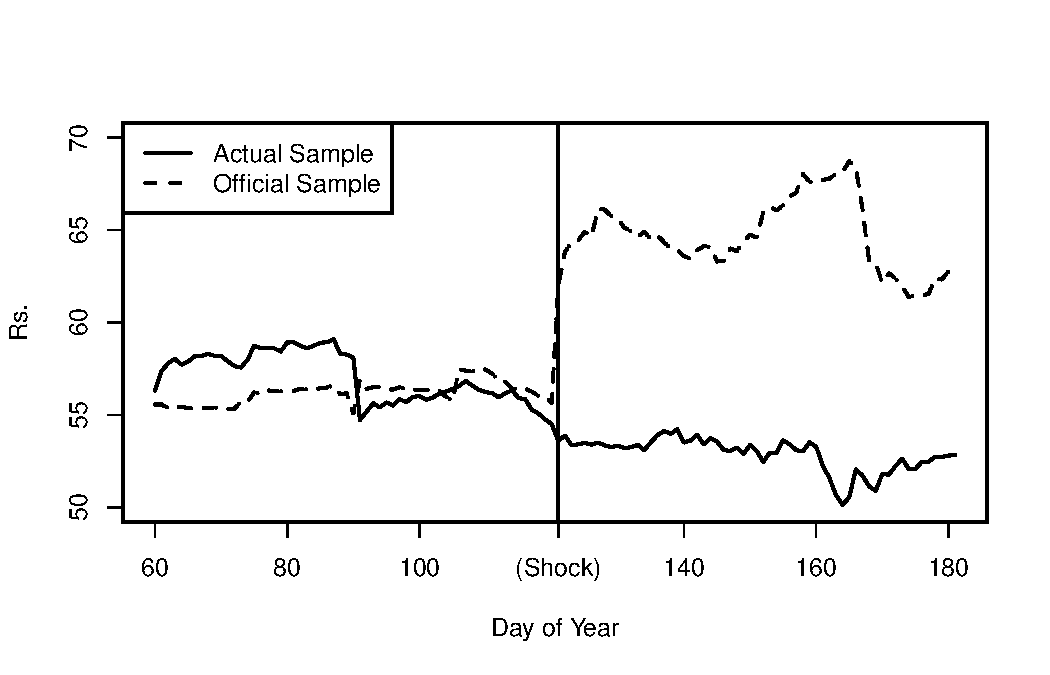
\includegraphics[scale=0.9]{wagetrends2.pdf}
\end{center}

In this graph, the data shows what happened when the wage shock policy was implemented. The actual sample shows the actual amount of work being done, the official sample shows the reported amount of work being done. Day 60 corresponds to March 1st, 2007, the start of the study period; day 121 to May 1st, 2007, the date of the wage shock; and day 181 to June 30, 2007, the end of the study period. As we can see on Day 60 when the wage increase policy happened, there was not an instant increase in official samples since the policy had not been implemented in all the panchayats yet. The shock happened on May 1, 2007, which had caused official samples to surge from Rs. 55 to Rs. 70 statutory wages. The officials deemed the risk of getting caught less than the profits that they would be earning due to the wage increase. While the actual amount of work that the people did was still around Rs. 55 range.
\subsection{Summary Statistics Table}
\begin{center}
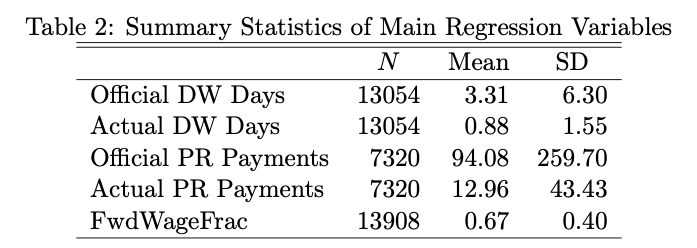
\includegraphics[scale=0.45]{Table2.png}
\end{center}

\subsection{Analysis for Replicated Statistics Table}
\begin{table}[!htbp] \centering 
  \caption{Summary Statistics of Main Regression Variables} 
  \label{} 
\begin{tabular}{@{\extracolsep{5pt}} cccc} 
\\[-1.8ex]\hline 
\hline \\[-1.8ex] 
 & Observations & Mean & St. Dev \\ 
\hline \\[-1.8ex] 
Official DW Days & 13054 & 3.31 & 6.30 \\ 
Actual DW Days & 13054 & 0.88 & 1.55 \\ 
Official PR Payments & 7320 & 94.08 & 259.70 \\ 
Actual PR Payments & 7320 & 12.96 & 43.43 \\ 
FwdWageFrac & 13908 & 0.67 & 0.40 \\ 
\hline \\[-1.8ex] 
\end{tabular} 
\end{table} 
 
In the table the "\emph{Offical DW Days} is the days worked by \emph{panchayat-day} on wage projects as reported officially. "Official PR Rate" is the total payments by \emph{panchayat-day} on wage projects as reported officially. "\emph{Actual DW Days}" is the days worked by \emph{panchayat-day} on daily wage projects as reported by survey respondents. "Official PR Rate" is the total payments by \emph{panchyat-day} on piece rate projects as reported officially. The "Actual PR Rate" Corresponds to the same figure as reported by survey respondents. "\emph{FwdWageFrac}" is the proportion of project days in the two months in a \emph{panchayat} that are daily wage.
 \newline 
 \newline
Our table looks exactly the same as the one in the original. We used the code and the data that was provided with the data using openICPSR.org but instead of using the latex converter that they had in the document, we supplemented it with Stargazer which provided the same summary statistics table. However, we changed the labeling of observations from N to Observations and labeling standard deviation from SD to St. Dev. 


\subsection{Regression Empirical Analysis}
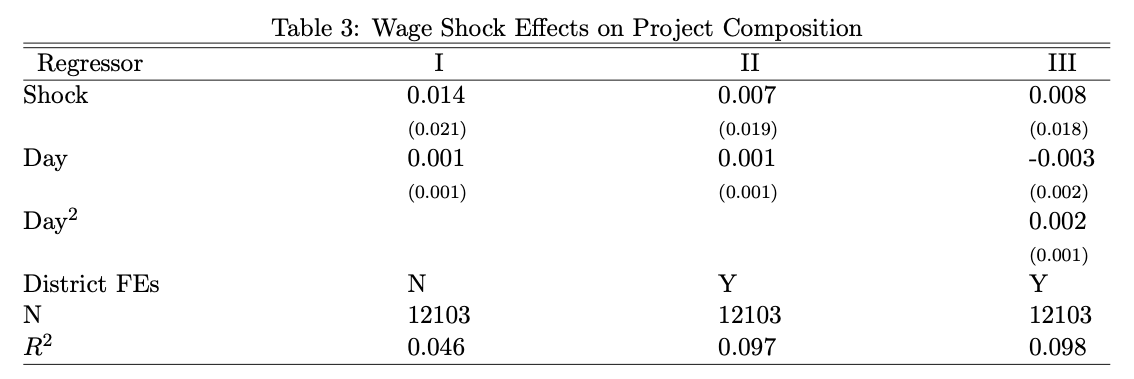
\includegraphics[scale=0.42]{Regression.png}
Statistical significance is denoted as: $*p < 0.10, **p < 0.05, ***p < 0.01$
\newline

Each observation is a \emph{panchayat-day} (the officially reported amount of output or the wage record of the local level government that the government has paid for each panchayat per day). The dependent variable in all regressions is “\emph{FwdWageFrac}”, the proportion of daily wage project-days in the \emph{panchayat} in the next two months. “Shock” is an indicator equal to 1 on and after May 1, 2007. “Day” is a linear time trend; Day2 has been re-scaled by the mean of Day. All columns include a third-order polynomial in the day of the month and indicators for major agricultural seasons. Robust standard errors multi-way clustered by \emph{panchayat} and day are presented in parenthesis. 

We were able to replicate almost exactly what the original table had. Apart from being able to replicate the standard errors, we were able to replicate every other part of the table. This was due to a function not working in the code that we received for the replication paper.  

If we did not have the code provided, we believe that it would be not very difficult to replicate the regression table since we are doing a multi-linear regression. We would just take the regression of the left-hand side variable to the right-hand side variables, which are the dependent variables, such as shock, day, $day^2$ which is the mean of the day data and the control variables, which were fixed district effects, holidays, the different reservations that people had about gender, the tribes, sbc, the different seasons during that time frame, and the day of the 3 months in the data set. Next, we used Stargazer in the code to find our variables and then put them in the table. The difficult part would have been how to put the data together from various sources and cleaning it so that it can be used. If we did not have the cleaned data provided by the people, it would have taken an extensive amount of time before even starting to code the items. The results would have been the same as shown with our replication in the table below. 



\begin{table}[!htbp] \centering 
  \caption{Wage Shock Effects on Project Composition} 
  \label{} 
\begin{tabular*}{\textwidth}{@{\extracolsep{\fill}}llll}\hline\hline
\multicolumn{1}{l}{Regressor}&\multicolumn{1}{c}{I}&\multicolumn{1}{c}{II}&\multicolumn{1}{c}{III}\tabularnewline
\hline
Shock&0.014$^{}$&0.007$^{}$&0.008$^{}$\tabularnewline
&{\scriptsize (0.015)}&{\scriptsize (0.015)}&{\scriptsize (0.015)}\tabularnewline
Day&0.001$^{}$&0.001$^{}$&-0.003$^{}$\tabularnewline
&{\scriptsize (0.0002)}&{\scriptsize (0.0002)}&{\scriptsize (0.001)}\tabularnewline
Day$^2$&&&0.002$^{}$\tabularnewline
&&&{\scriptsize (0.0004)}\tabularnewline
District FEs&N&Y&Y\tabularnewline
N&12103&12103&12103\tabularnewline
$R^2$&0.046&0.097&0.098\tabularnewline
\hline
\end{tabular*}
\end{table}



\subsection{Hypothesis Testing For Original Regression}
To help further explain that there is a relationship, the officially reported wage hours and the wage increase shock, we decided to do a hypothesis testing upon the original population regression function:

\begin{center}
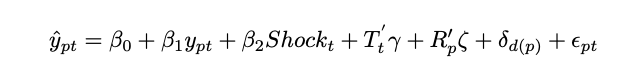
\includegraphics[scale=0.5]{OEQ.png}
\end{center}
\newline
For hypothesis testing they define the null and alternative as:
\newline
$$H_0: B_2 < C$$
$$H_1: B_2 > C$$
\begin{center}
Where C is the critical value.
\end{center}

We define $B_2$ as Shock.To test this hypothesis we will find our critical value,first finding the degrees of freedom using this function: 
$$df = N-R-1$$
$$df = 12103 - 13 -1$$ 
$$df = 12,089$$ 
With the degrees of freedom being $12,089$, then we set $\alpha = 0.05$. Using the one tail test we will find that our critical value is $1.65$.
\newline
\newline
Next we will use the the function to calculate our t-statistical which is:
$$T-stat = \frac{\hat{\beta}-B_0}{SE(\hat{\beta})} $$

Column I $\beta_2$ (\emph{Shock}) was $0.6667$, Column II $\beta_2$  was $0.3684$,and Column III $\beta_2$ was $0.444$. Since $\beta_2$ is less than the critical value of $1.65$. $\beta_2$ fails to reject the null, thus proving and disproving a definite relationship, failing to reject the null indicates that the sample did not provide enough evidence to conclude that the effect exists. At the same time, the lack of evidence doesn't prove that the effect does not exist. 
This therefore states that the wage increase policy was insignificant to the overall wage project composition. Meaning that this wage increase policy shock in May 1, 2007 had little to none overall effect to decreasing corruption among the panchayat officials.
\subsection{Hypothesis Testing For Replicated Regression}
Now we will repeat the process for our replicated regression to see if we also get the same results as the original paper. Our PRF does not change and remains the same.
$$\hat{y}_{pt}= \beta_0 + \beta_1 y_{pt} + \beta_2Shock_t + T^{'}_t\gamma + R^{'}_p\zeta  + \epsilon_{pt}  $$
\newline
For hypothesis testing we define the null and alternative as:
\newline
$$H_0:B_2 < C$$
$$H_1:B_2 > C$$
\begin{center}
Where C is the critical value
\end{center}

We will repeat the same process as before and to calculate our critical value
which is $1.65$. Next, we will repeat the process to find our t-stats, using our replication data. For our Column I $\beta_2$ (\emph{Shock}) was $0.924$, Column II $\beta_2$  was $0.493$,and Column III $\beta_2$ was $0.542$. Just like the original hypothesis, $B_2$ failed to reject the null due to the sample not having enough evidence to prove or disprove a definite relationship. 

The original paper had stated that their results said "regressions of \emph{FwdWageFrac} on an indicator for the shock along with time controls. The point estimates are insignificant and correspond to a 0.02 standard deviation change in project composition". The table shows the $R^2$ which shows a very low significance level but through hypothesis testing, we found out that \emph{panchayat-day} shows a high significance with the dependent variables $"FwdWageFrac"$ and $Day$ . But since for the variable $Shocks$ we could not prove or disprove for a relationship. We have the same results as the original paper thus this tells us that the wage increase policy did not decrease corruption. 


\section{Conclusion}
In conclusion, in this replication paper, we were looking into how effective the wage increase policy was in decreasing the amount of corruption being committed by the officials of the panchayat. Though replicating the paper, we identified that there was a small and weak significance with how the wage increase policy helped with decreasing corruption. We believe this was due to this being a 3-month study. We believe that if this study took place for longer than a year and this wage increase policy was permanent, the panchayat officials would see that the wage increase policy as a goose who lays golden eggs. Thus decreasing corruption since they would not want to kill the goose that lays the golden eggs.

Though replicating the paper we realized the limitations for replicating the paper. Since the code that was provided was old, some code functions did not work the same anymore. Therefore we had to think outside the box and substitute the function for another. If the paper did not come with R code or cleaned data sets, another limitation we would have run into was that most paper codes are written in Stata. It would have been very difficult to translate the Stata code to R code. The previous papers that we tried to replicate gave us this problem. Some parts of the Stata code proved that we would need at least 2 to 3 weeks to translate the code before we even start typing the paper. The next limitation we would have run into is cleaning the data; the paper provided a fully cleaned data set. Our first paper took over 60 hours to clean 80\% of our data, and we realized that cleaning data takes a great deal of time. We are very grateful for the authors including the cleaned data table to make the replication process run more smoothly. All through this paper was challenging, it made us realize the many difficulties of a proper economics paper. 

\section{References}
(1)
Niehaus, Paul, and Sandip Sukhtankar. “Corruption Dynamics: The Golden Goose Effect.” American Economic Journal: Economic Policy 5, no. 4 (November 2013): 230–69. https://doi.org/10.1257/pol.5.4.230.

\end{document}
